
\chapter{Interface homme machine}

\section{Fonctionnalités de l' IHM}

L'interface homme-machine est un des composant essentiel de notre projet. En effet, c'est grâce à elle que l'utilisateur va pouvoir juger de la qualité du logiciel. Ainsi, conformément au  cahier des charges, on va retrouver les fonctionnalités suivantes :

\begin{itemize}
 \item Explorateur de documents
\begin{itemize}
 \item Module
 \item Dossier
 \item Cours
\end{itemize} 
 \item Visualisation du cours
 \item Editeur de texte
\begin{itemize}
 \item Outils de formatage
 \item Affichage du plan 
\end{itemize} 
 \item Export au format PDF
 \item Export/import au format RTF (Format Microsoft)
 \item Impression du cours édité

\end{itemize}



\section{Ergonomie}

\subsection{Solutions de visualisation et d'édition envisagées}

En ce qui concerne l'ergonomie du logiciel plusieurs choix de conception ont été mis en confrontation. Le premier, qui n'a finalement pas été retenu était d'utiliser un unique éditeur de texte. Celui-ci aurai joué un  double rôle, tout d'abord celui d'un panneau de visualisation du cours, prononcé par l'enseignant. Le cours aurai été affiché à la fin du document. De plus, l'utilisateur aurai eu la possibilité de modifier le panneau de visualisation dans le but d'organiser son  cours.

Le principal soucis de cette solution était que le travail de restructuration du cours en direct aurai été une tâche particulièrement fastidieuse et aurai fortement perturber la suivie du cours.

Ainsi, la solution finalement envisagée est l'utilisation de deux panneaux. Un premier dont le but est d'afficher le texte brut issu du moteur de reconnaissance vocale. Celui-ci à pour but de permettre à l'utilisateur mal entendant d'utiliser sa  vision en remplacement. Le second panneau lui à pour but de servir de support de cours, offrant la possibilité de prise de notes. De la même façon qu'un étudiant normal prendrai des notes sur papier.

Bien que cette solution semble la plus productive et la plus intéressante, elle est n'est pas exempt de défauts. Ainsi, il faut bien souligner le fait qu'il est particulièrement difficile de lire un texte tout en réalisant des  prises de notes.     



\subsection{Accessibilité}

Un des points fondamentaux de l'IHM était de concevoir une interface facile d'utilisation et un maximum intuitive. Ainsi, un effort particulier à été réalisé de façon à ce que l'utilisateur prenne rapidement en main l'outil. Pour cela différents points ont étés réalisés :

\begin{itemize}
 \item Une barre d'outils avec des icônes explicites : pour permettre un accès rapide au principales fonctions
 \item Création de raccourcis claviers classiques (CTRL-C, CTRL-V ...)
 \item Utilisation des standards d'ergonomie : Placement des menus, des boutons ...
\end{itemize}



\section{Conception MVC}


\begin{figure}[h]
 \centering
 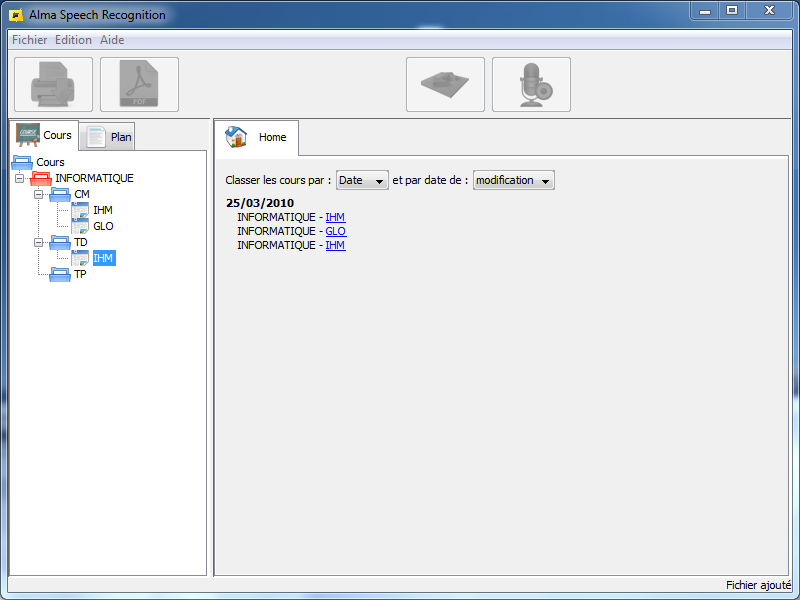
\includegraphics[scale=0.6]{./images/homePanel.png}
 % homePanel.png: 0x0 pixel, -2147483648dpi, 0.00x0.00 cm, bb=
 \caption{IHM - Panneau d'accueil}
 \label{fig:homePanel}
\end{figure}



\begin{figure}[h]
 \centering
 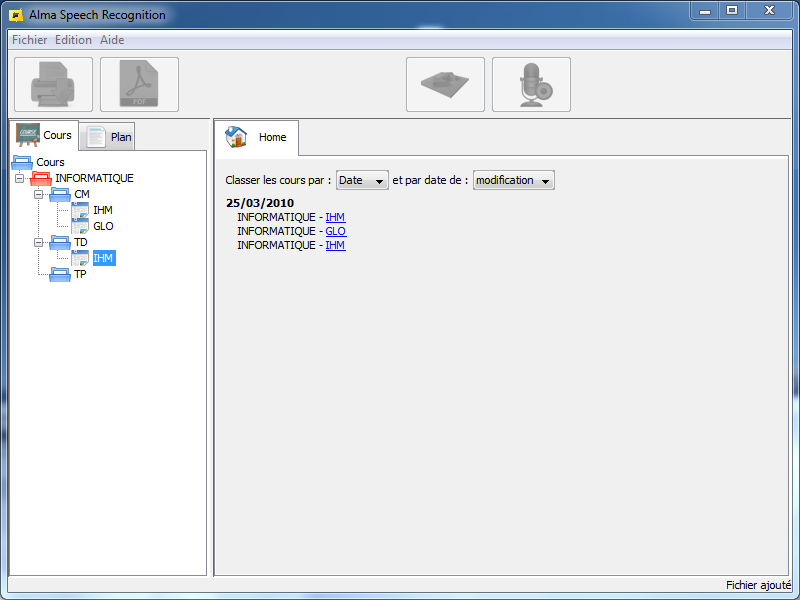
\includegraphics[scale=0.6]{./images/homePanel.png}
 % homePanel.png: 0x0 pixel, -2147483648dpi, 0.00x0.00 cm, bb=
 \caption{IHM - Panneau de travail}
 \label{fig:homePanel}
\end{figure}
